\documentclass{book}
\usepackage[ngerman]{babel}
\usepackage[utf8]{inputenc}
\usepackage{fancyhdr}
\usepackage{amsmath}
\usepackage{amsthm}
\usepackage{amssymb}
\usepackage{amsfonts}
\usepackage{mathtools}
\usepackage{xhfill}
\usepackage{xcolor}
\usepackage{graphicx}
\usepackage{float}
\usepackage{esint}
\usepackage{hyperref}
\usepackage[most]{tcolorbox}
\usepackage[chapter]{algorithm}
\usepackage{algpseudocode}


\graphicspath{ {./imgs/} }
\usepackage[
  a4paper,
  textwidth=175mm,
  textheight=225mm,
  heightrounded,
]{geometry}

\pagestyle{fancy}
\lhead{}
\chead{\thechapter. \chaptername}
\rhead{}
\lfoot{}
\cfoot{\thepage}
\rfoot{}

\author{Manuel Hinz}

\title{Einführung in die Grundlagen der Numerik (WS 22/23)}

\newtheorem{theorem}[algorithm]{Satz}
\newtheorem{corollary}[algorithm]{Korollar}
\newtheorem{lemma}[algorithm]{Lemma}
\newtheorem{definition}[algorithm]{Definition}
\newtheorem{remark}[algorithm]{Bemerkung}
\newtheorem*{mremark}{Eingefügte Bemerkung}
\newtheorem{example}[algorithm]{Beispiel}
\newtheorem*{mdefinition}{Eingefügte Definition}
\newtheorem*{mexample}{Eingefügtes Beispiel}



\def\C{\mathbb{C}}
\def\R{\mathbb{R}}
\def\N{\mathbb{N}}
\def\Z{\mathbb{Z}}
\def\rang{\text{rang}}
\def\cond{\text{cond}}
\def\eps{\text{eps}}
\raggedright

\let\cleardoublepage=\clearpage

\begin{document}

    \maketitle

    \tableofcontents

    \section*{Vorwort}

            Diese Mitschrift von der Vorlesung Einführung in die Grundlagen der Numerik (Dölz,WS 2022/2023) 
            wird von mir neben der Vorlesung geschrieben und ist dementsprechend Fehleranfällig. Fehler gerne an 
            mh@mssh.dev! 

    \chapter{Orthogonalität}

        \section{Grundlegende Definitionen}

            \begin{definition}\label{d1.1}
                Sei $X$ ein $\R$ Vektorraum und $\langle\cdot,\cdot\rangle:X\times X \to \R$ eine Abbildung. $\langle\cdot,\cdot\rangle$ heißt \textbf{Skalarprodukt} oder inneres Produkt, falls
                \begin{equation}
                    \tag{Positiviät}
                    \forall f\in X\setminus 0: \langle f,f \rangle>0
                \end{equation}
                \begin{equation}
                    \tag{Symmetrie}
                    \forall f,g\in X: \langle f,g \rangle = \langle g,f \rangle
                \end{equation}
                \begin{equation}
                    \tag{Linearität im ersten Argument}
                    \forall \alpha,\beta\in\R, f,g,h\in X: \langle \alpha f+\beta g,h \rangle
                    = \alpha \langle f,h \rangle + \beta \langle g,h \rangle
                \end{equation}
            \end{definition}

            \begin{remark}\label{b1.2}
                Symmetrie und Linearität im ersten Argument implizieren, 
                dass $\langle \cdot,\cdot  \rangle$ eine bilineare Abbildung ist. 
            \end{remark}

            \begin{definition}\label{d1.3}
                Sei $X$ ein $\R$-Vektorraum mit Skalarprodukt $\langle \cdot,\cdot \rangle$.
                Wir bezeichnen die zugehörige \textbf{Norm} (in Abhänigkeit von einem Vektor $f\in X$) mit 
                \begin{equation*}
                    \Vert f \Vert =\sqrt{\langle f,f\rangle}.
                \end{equation*}
            \end{definition}

            \begin{lemma}\label{l1.4}
                Sei $X$ ein $\R$-Vektorraum mit Skalarprodukt $\langle \cdot,\cdot \rangle$. Dann gil die \underline{Cauchy-Schwarz-Ungleichung}:
                \begin{equation}
                    \tag{C.S.}
                    \forall f,g\in X:\langle f,g \rangle\leq \Vert f\Vert \cdot\Vert g \Vert
                \end{equation}
                mit Gleichheit genau dann, wenn $f$ und $g$ linear abhängig sind.
            \end{lemma}
            \begin{proof}
                O.B.d.A. $f,g\neq 0$, da sonst offensichtlich Gleichheit gilt.
                Sei $\alpha\neq 0$, dann gilt mit $f,g\in X$ und $\alpha \in \R$:
                \begin{equation*}
                    0\leq \Vert f -\alpha g\Vert^2= \langle f-\alpha g,f-\alpha g \rangle
                    = \Vert f \Vert^2 -2\alpha \langle f,g \rangle+\alpha^2 \Vert g \Vert^2
                \end{equation*}
                Wählen wir jetzt $\alpha=\frac{\langle f,g \rangle}{\Vert g \Vert^2}$ folgt:
                \begin{equation*}
                    0\leq \Vert f \Vert^2-\frac{2 \langle f,g \rangle^2}{\Vert g \Vert^2}+\frac{\langle f,g \rangle^2}{\Vert g \Vert^2}
                \end{equation*}
                \begin{equation*}
                    \implies \langle f,g \rangle^2\leq \Vert f \Vert^2\cdot \Vert g \Vert^2.
                \end{equation*}
            \end{proof}
            \begin{mremark}
                Rechnung zur Begründung von $ \langle f-\alpha g,f-\alpha g \rangle
                = \Vert f \Vert^2 -2 \Vert\alpha \langle f,g \rangle+\alpha^2 \Vert g \Vert^2$:
                \begin{align*}
                    &\langle f-\alpha g,f-\alpha g \rangle\\
                    &=\langle f,f-\alpha g \rangle-\alpha \langle g,f-\alpha g \rangle\\
                    &=\langle f,f \rangle-\alpha \langle f,g \rangle-\alpha \langle g,f \rangle+\alpha^2 \langle g,g \rangle\\
                    &=\Vert f \Vert^2 -2 \Vert\alpha \langle f,g \rangle+\alpha^2 \Vert g \Vert^2
                \end{align*}
            \end{mremark}
            \begin{example}\label{b1.5}
                \begin{enumerate}
                    \item $X=\R^n$ und $\langle x,y \rangle=\sum_{i=1}^n x_iy_i$ (Euklidisches Skalarprodukt)
                    \item $X=\R^n$, $\langle x,y \rangle=x^\perp A y$, wobei $A$ positiv definit und symmetrisch ist
                    \item $I=[a,b],w:I\to\R$ beschränkt und strikt positiv:
                        \begin{equation*}
                            X=\left\{f:I\to\R:\int_a^b f(x)^2w(t)dt<\infty\right\}=L^2(I,w)
                        \end{equation*}
                        mit 
                        \begin{equation*}
                            \langle f,g \rangle = \int_a^b f(t)g(t)w(t)dt
                        \end{equation*}
                \end{enumerate}
            \end{example}
            \begin{mremark}
                Die Definition von $L^2(I,w)$ ist hier nicht ganz richtig, man müsste natürlich noch Äquivalenzklassen, bzgl. Gleichheit bis auf Nullmengen, bilden. 
                Dies wird hier, da Analysis 3 / Wtheo. nicht nicht vorrausgesetzt wird, ignoriert.
            \end{mremark}
            \begin{definition}\label{d1.6}
                Sei $X$ ein $\R$-VR mit Skalarprodukt $\langle \cdot,\cdot \rangle$.
                $f,g\in X$ heißen \textbf{orthogonal}, falls $\langle f,g \rangle=0$.
            \end{definition}
            \begin{remark}\label{b1.7}
                Im $\R^n$ mit dem euklidischen Skalarprodukt stimmt Definition \ref*{d1.6}, wegen 
                \begin{equation*}
                    \langle x,y \rangle = \Vert x \Vert \Vert y \Vert \cos(\theta), \theta=\angle(x,y),
                \end{equation*}
                mit unserem bisherigen Verständnis überein.
            \end{remark}
        \section{Bestapproximationseigenschaft}
            \begin{definition}\label{d1.8}
                Sei $V$ ein $\R$-VR mit Skalarprodukt $\langle \cdot,\cdot \rangle$ und $U$ ein Unterraum.
                \begin{equation*}
                    U^\perp = \left \{ v\in V: \langle v,u \rangle=0,\forall u\in U\right\}
                \end{equation*}
                heißt das \textbf{orthogonale Komplement} von $U$.
            \end{definition}
            \begin{theorem}\label{s1.9}
                Unter den Annahmen von Definition \ref*{d1.8} und der  zusätzlichen Annahme, dass $U$ endlich dimensional ist, gilt folgendes für $v\in V$:
                \begin{equation*}
                    \Vert v-u \Vert = \min_{w\in U}\Vert v-w\Vert
                \end{equation*}
                genau dann, wenn $v-u\in U^\perp$.
            \end{theorem}
            \begin{example}\label{b1.10}
                $V=\R^2$, $U=\text{span}\left\{\begin{pmatrix}1\\1\end{pmatrix}\right\}$ mit euklidischem Skalarprodukt $\langle \cdot,\cdot \rangle$.
                Dann ist $U^\perp = \text{span}\left\{\begin{pmatrix}1\\-1\end{pmatrix}\right\}$. 
                \begin{figure}[H]
                    \centering
                    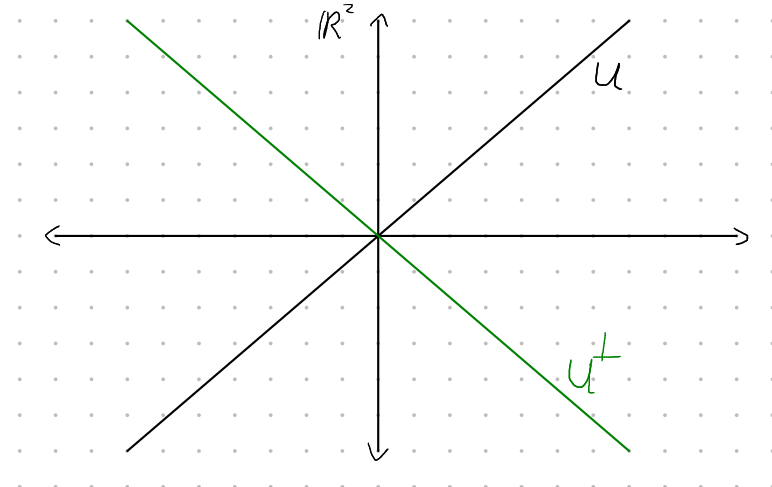
\includegraphics[width=0.25\textwidth]{Bild001}
                    \caption{\(U\) und \(U^\perp\)}
                \end{figure}
            \end{example}
            \begin{proof}[Beweis von Satz \ref*{s1.9}]
                Sei $v\in V$ und seien $u,w\in U$. Dann gilt:
                \begin{equation*}
                    \Vert v-w \Vert^2=\langle v-w,v-w \rangle = \langle (v-u)+(u-w),(v-u)+(u-w) \rangle
                \end{equation*}
                \begin{equation*}
                    =\Vert v-u \Vert^2+2 \langle v-u,\underbrace{u-w}_{\in U} \rangle +\Vert u-w \Vert^2\geq \Vert v-u \Vert^2
                \end{equation*}
                mit Gleichheit genau dann, wenn $w-u=0$ (da dann der $\Vert u-w \Vert$ Term verschwindet).
            \end{proof}
            \begin{remark}\label{b1.11} 
                Der Satz sagt, dass es zu \underline{jedem} $v\in V$ ein \underline{eindeutiges, bestmögliches} $u\in U$ gibt.
            \end{remark}
            \begin{definition}\label{d1.12} 
                Die Lösung aus Satz \ref*{s1.9} heißt \textbf{orthogonale Projektion} von $v$ auf $U$. Die Abbildung 
                \begin{equation*}
                    P:V\to U, v\mapsto P(v) \textbf{ mit } \Vert v-Pv \Vert=\min_{w\in U}\Vert v-w \Vert
                \end{equation*}
                ist linear und wird \textbf{orthogonale Projektion} genannt.
            \end{definition}
            \begin{mremark}[Beweis der Linearität]
                Für $v_1,v_2\in V$ und $\alpha\in \R$ gilt:
                \begin{align*}
                    v_1-Pv_1\in U^\perp\\
                    v_2-Pv_2\in U^\perp 
                \end{align*}
                Daher 
                \begin{align*}
                    \alpha(v_1-Pv_1)+(v_2-Pv_2)=(\alpha v_1+v_2) - (\alpha Pv_1 + Pv_2) \in U^\perp.
                \end{align*}
                Aber dann muss $\alpha Pv_1+Pv_2$ schon, wegen der Eindeutigkeit, $P(\alpha v_1+v_2)$ sein.
            \end{mremark}
            \begin{remark}\label{b1.13}
                Satz \ref{s1.9} gilt auch, wenn $U$ durch $W=w_0+U$ ersetzt wird.
                Die orthogonale Projektion ist analog definiert..
            \end{remark}

            \underline{\textbf{Frage:}} Die Orthogonale Projektion hat offenbar gute Eigenschaften. Aber: wie berechnen wir sie? Wie wählen wir $U$?
            
            \begin{itemize}
                \item Berechnung ist leicht
                \item U wählen schwierig
            \end{itemize}

        \section{Orthonormalbasen}

            \begin{definition}\label{d1.14}
                Sei $X$ ein $\R$-VR mit Skalarprodukt $\langle \cdot,\cdot \rangle$ und
                $X_n\subset X$ ein endlich dimensionaler Teilraum mit Basis $\{\varphi_1,\dots,\varphi_n\}$.
                Die Basis heißt \textbf{Orthogonalbasis}, falls 
                \begin{equation*}
                    \forall i\neq j: \langle \varphi_i,\varphi_j \rangle=0
                \end{equation*}
                gilt und Orthonormalbasis (ONB), falls zusätzlich $\Vert\varphi_i\Vert=1$ gilt. Das impliziert:
                \begin{equation*}
                    \langle \varphi_i,\varphi_j \rangle =\delta_{i,j}.
                \end{equation*}
            \end{definition}

            \begin{example}\label{b1.15}    
                \begin{enumerate}
                    \item $\R^n$ mit euklidischem Skalarprodukt und kanonischer Basis
                    \item $X=L^2(I,1)$ mit entsprechendem Skalarprodukt und $X_n$ der Raum der trigonometrischen Polynome bis Grad $n$.
                    Dann ist folgendes eine ONB:
                    \begin{equation*}
                        \left\{\frac{1}{\sqrt{2\pi}},\frac{\sin(x)}{\sqrt{\pi}},\frac{\cos(x)}{\sqrt{\pi}},\dots,\frac{\sin(nx)}{\sqrt{\pi}},\frac{\cos(nx)}{\sqrt{\pi}}\right\}
                    \end{equation*}
                \end{enumerate}
            \end{example}

            \begin{mremark}
                Trigonometrische Polynome sind Funktionen der Form
                \begin{equation*}
                    f(t)=\sum_{k=1}^n a_k \cos(kx)+ b_k \sin(kx).
                \end{equation*}
                Die größte Faktor vor dem $x$ ist der Grad eine trigonometrischen Polynoms.
            \end{mremark}

            \begin{theorem}\label{s1.16}
                Sei $\{\varphi_1,\dots,\varphi_n\}$ eine ONB von $X_n\subset X$. Dann gilt
                \begin{enumerate}
                    \item $f=\sum_{i=1}^n \langle \varphi_i,f \rangle\varphi_i$
                    \item $\Vert f \Vert^2=\sum_{i=1}^n \langle \varphi_i,f \rangle^2$
                    \item Die orthogonale Projektion $f_n$ von $f\in X\setminus X_n$ ist gegeben durch 
                        \begin{equation*}
                            f_n=\sum_{i=1}^n \langle \varphi_i,f \rangle\varphi_i
                        \end{equation*}
                    \item im Fall von 3.:
                        \begin{equation*}
                            \Vert f_n \Vert^2 = \sum_{i=1}^n \langle \varphi_i,f \rangle^2 \leq \Vert f \Vert
                        \end{equation*}
                \end{enumerate}
            \end{theorem}
            
            \begin{proof}
                1.: 
                \begin{align*}
                    &f\in X_n\implies \exists \alpha_i\in \R: f=\sum_{i=1}^n\alpha_i\varphi_i\\
                    &\implies \langle \varphi_i,f \rangle= \langle \varphi_i, \sum_{j=1}^n\alpha_j\varphi_j\rangle
                    =\sum_{j=1}^n \alpha_j \langle \varphi_i,\varphi_j \rangle =\alpha_i
                \end{align*}
                2.:
                \begin{align*}
                    &\Vert f \Vert^2 = \langle f,f \rangle \\
                    &= \langle \sum_{i=1}^n \alpha_i \varphi_i, \sum_{j=1}^n \alpha_j \varphi_j \rangle =\sum_{i,j=1}^n\alpha_i\alpha_j\delta_{i,j}=\sum_{i=1}^n\alpha_i^2
                \end{align*}
                3.:
                \begin{align}
                    f\in X\setminus X_n:&\nonumber\\
                    \Vert f-\underbrace{\tilde{f}_n}_{\in X_n} \Vert &= \langle f-\sum_{i=1}^n\tilde{\alpha}_i\varphi_i,f-\sum_{i=1}^n\tilde{\alpha}_i\varphi_i \rangle\nonumber\\
                    &=\Vert f \Vert^2-2\sum_{i=1}^n\tilde{\alpha}_i \underbrace{\langle \varphi_i,f \rangle}_{\eqqcolon \alpha_i}+\sum_{i,j=1}^n\alpha_i\alpha_j \langle \varphi_i,\varphi_j \rangle \nonumber\\
                    &=\Vert f \Vert^2-\sum_{i=1}^n\tilde{\alpha}_i\alpha_i+\sum_{i=1}^n\tilde{\alpha}_i^2
                    \stackrel{\text{Quadratische Ergänzung}}{=} \Vert f \Vert^2-\sum_{i=1}^n\alpha_i^2+\sum_{i=1}^n\underbrace{(\alpha_i-\tilde{\alpha}_i)^2}_{\geq 0}
                \end{align}
                Dies wird minimiert, wenn $\tilde{\alpha}_i=\alpha_i$ ist.
                
                4.:

                $f\in X_n$ wurde in 2. gezeigt. Sonst:
                \begin{equation*}
                    f\notin x_n\implies \text{ mit } \alpha_i=\tilde{\alpha}_i \text{ in } (1.1):
                \end{equation*}
                \begin{equation*}
                    0\leq \Vert f-f_n \Vert^2=\Vert f \Vert^2-\sum_{i=1}^n\underbrace{\alpha_i^2}_{\langle \varphi_i,f \rangle^2}
                \end{equation*}
                Es folgt die Behauptung.
            \end{proof}

            \underline{\textbf{Vorteile von Orthogonalität:}}
            \begin{itemize}
                \item Bestapproximation
                \item Einfache Basisdarstellung
            \end{itemize}

        \noindent
        \xrfill[0.7ex]{1pt}Ende von Vorlesung 01 am 11.10.2022\xrfill[0.7ex]{1pt}

    \chapter{Das lineare Ausgleichsproblem}

        \section{Problemstellung und Normalengleichung}

            Gegeben seien Punkte $(t_i,b_i)\in\R^2$ mit $i=1,\dots,m$. Wir nehmen an, dass es eine Gestzmäßigkeit im Sinne eines
            parameterabhängigen Modelles 
            \[
                b_i=b(t_i)=b(t_i;\underbrace{x_1,\dots,x_n}_{\text{Parameter}}),
            \]
            wobei die Parameter $x_1,\dots,x_n$ unbekannt seien, gibt. In der Praxis sind die Messungen zusätzlich mit Fehlern
            behaftet und das Modell gilt nur approximativ. Zusätzlich gibt es oft mehr Messungen als Parameter, d.h. $m>n$.

            \underline{\textbf{Frage:}} Gegeben die Messungen, können wir zugehörige Parameter bestimmen?

            \underline{\textbf{Annahme:}} $b$ ist linear in den Parametern, d.h. es gibt Funktionen 
            \[a_i:\R\to\R\]
            s.d.
            \[b(t;x_1,\dots,x_n)=a_1(t)x_1+\dots+a_n(t)x_n.\]
            \underline{\textbf{Idee:}} Formuliere ein lineares Gleichungssystem:
            \[b_i \approx b(t_i;x_1,\dots,x_n)=a_1(t_i)x_1+\dots+a_n(t_i)x_n, i=1,\dots,m\]
            kurz $Ax\approx b$ mit $A\in\R^{m\times n},x\in\R^n,b\in\R^m$.

            \underline{\textbf{Problem:}} Durch Modell- und Messfehler gilt das Gleichungssystem nur ungefähr, und wir 
            mehr Gleichungen als Unbekannte (``das Gleichungssystem ist überbestimmt''). Wir können unser Gleichungssystem 
            also im Allgemeinen nicht lösen.

            \begin{example}\label{b2.1}
                \begin{figure}[H]
                    \centering
                    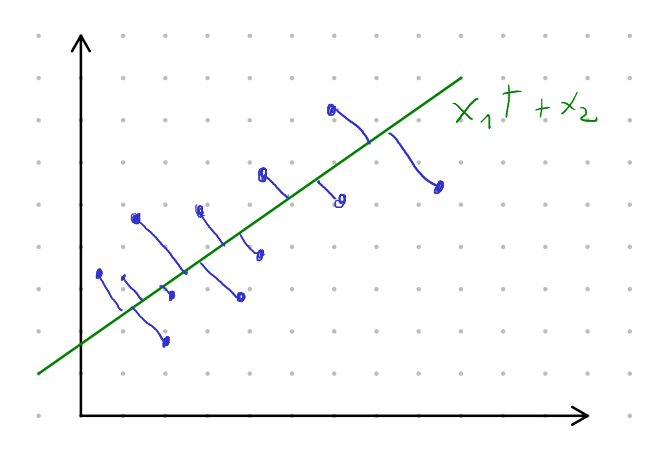
\includegraphics[width=0.25\textwidth]{Bild002}
                    \caption{Datenpunkte und approximierte Gerade}
                \end{figure}
            \end{example}

            \underline{\textbf{Idee:}} Finde Parameter, sodass das Modell ``bestmöglich'' mit den Messpunkten übereinstimmt, 
            d.h. finde $(x_1,\dots,x_n)^t=x\in\R^n$ s.d.:
            \begin{equation}\label{g2.1}
                \Vert Ax-b \Vert=\min_{y\in\R^n} \Vert Ay-b \Vert
            \end{equation}
            
            \begin{definition}\label{d2.2}
                Die Gleichung (\ref{g2.1}) heißt \textbf{lineares Ausgleichsproblem}. Der Term $Ax-b$ heißt \textbf{Residuum}.
            \end{definition}

            \underline{\textbf{Bemerke:}} $V=\R^m,U=\text{Bild}(A)\subset V,\dim(\text{Bild}(A))\underbrace{\leq n\leq m}_{\text{Grundannahme}}$

            Statte $V$ mit euklidischem Skalarprodukt aus.

            $\stackrel{Satz \ref{s1.9}}{\implies}$ Es gibt genau ein $Ax\in$ Bild$(A)$ so, dass
            \[\Vert Ax-b \Vert=\min_{w\in U} \Vert w-b \Vert\]
            gilt.

            \underline{\textbf{Aber:}} Wie berechnen wir $x$?

            \begin{theorem}\label{s2.3}
                Sei $A\in\R^{m\times n},b\in\R^m,m\geq n,x\in\R^n$ ist genau dann eine Lösung von (\ref{g2.1}) 
                bezüglich der euklidischen Norm, falls
                \begin{equation}\label{g2.2}
                    A^tAx=A^tb.
                \end{equation}
                Insbesondere ist das lineare Ausgleichproblem genau dann lösbar, falls $\rang(A)=n$.
            \end{theorem}

            \begin{proof}
                \begin{align*}
                    &\Vert Ax-b \Vert=\min_{y\in\R^n} \Vert Ay-b \Vert\\
                    &\stackrel{\text{Satz } (\ref{s1.9})}{\iff}Ax-b\in U^\perp=\text{Bild}(A)^\perp\\
                    &\iff \forall y\in\R^n: \langle Ax-b, Ay\rangle=0\\
                    &\iff \forall y\in\R^n: \langle A^tAx-A^tb,y \rangle=0\\
                    &\iff A^tAx=A^tb
                \end{align*}
                Die letzte Gleichung ist genau dann invertierbar, wenn $A^tA$ vollen Rang hat, also wenn $A$ vollen Rang ($n$) hat.
            \end{proof}

            \begin{remark}\label{b2.4}
                Im beweis verwenden wir, dass $Ax-b$ orthogonal zu $U=\text{Bild}(A)$,

                    \begin{figure}[H]
                        \centering
                        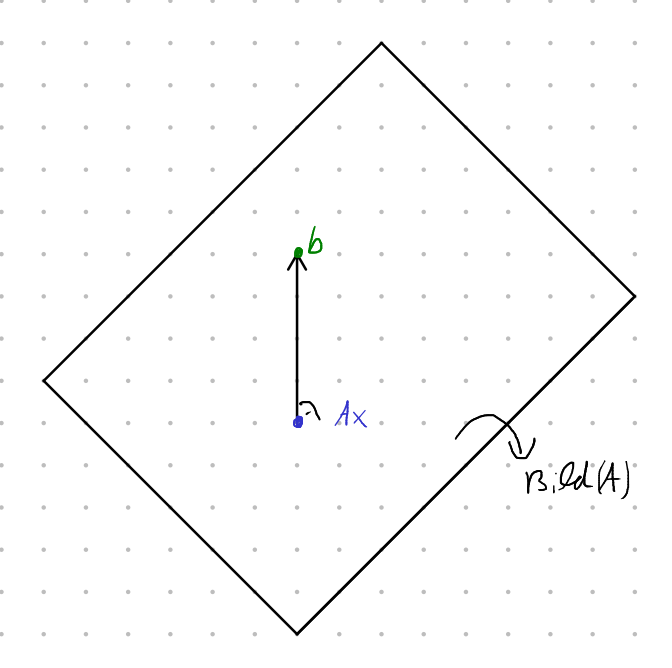
\includegraphics[width=0.25\textwidth]{Bild003}
                        \caption{Hyperebene und Projektion}
                    \end{figure}

                d.h. eine Normale zur Hyperebene Bild$(A)$ im $R^m$, ist. Deshalb heißt (\ref{g2.2}) auch \textbf{Normalengleichung}.
            \end{remark}

            \begin{remark}\label{b2.5}
                Für $m=n$ und $\rang(A)=n$ ist die Lösung des linearen Ausgleichproblems exakt (im mathematischen Sinne).
            \end{remark}

            \begin{theorem}\label{s2.6}
                Für $A\in\R^{m\times n}$ ist $A^tA$ symmetrisch und positiv semidefinit. Falls $m\geq n$ ist $A^tA$ genau 
                dann positiv definit, wenn $\rang(A)=n$.
            \end{theorem}
            \begin{proof}
                \begin{itemize}
                    \item Symmetrisch: klar
                    \item positiv semidefinit:
                    \[\forall x\in \R^n: x^t(A^tA)x=(Ax^t)(Ax)=\Vert Ax \Vert_2^2\geq 0\]
                    \item positiv definit: $\rang(A)=n\implies Ax=0\iff x=0\implies \Vert Ax \Vert_2=0\iff x=0\implies $ Behauptung.
                \end{itemize}
            \end{proof}
        
        Einfachste Möglichkeit zur Lösung von (\ref{g2.2}): Berechne $A^tA,A^tb$, löse LGS mittels Cholesky. Kosten sind ungefähr:
        \[\frac{n^2m}{2}+m\cdot n+\frac{n^3}{6}+\frac{n^2}{2}+\frac{n^2}{2}\approx\frac{mn^2}{2} \text{ für } m\gg n.\]
        
        \begin{mremark}
            Anmerkung vom Donzent: $A^tA$ eig. immer schlecht zu berechnen.
        \end{mremark}

        %Hier Konditionierung nacharbeiten

        \underline{\textbf{Aber:}} Dieser Vorgang ist schlechter konditioniert als das lineare Ausgleichsproblem: 
        
        \begin{tcolorbox}[enhanced,breakable,
            title=Eingeschobene Definition / Wiederholung]
            \[
                \cond(A)=\Vert A \Vert \Vert A^{-1} \Vert
            \]
            \[
                \Vert A \Vert =\max_{\Vert x \Vert=1} \Vert Ax \Vert
            \]
        \end{tcolorbox}

        Falls $A\in\R^{n\times n}$ spd (symmetrisch, positiv definit) gilt $\cond_2((A^tA))=\cond_2(A)^2$. 

        Für $A\in\R^{m\times n}$ gelten ähnliche Überlegungen, siehe Deuflhard \& Hohmann.

        \begin{example}\label{b2.7}
            Sei $A=\begin{bmatrix}
                1 & 1\\\epsilon&0\\0 & \epsilon
            \end{bmatrix}$ mit $\epsilon>\underbrace{\eps}_{\text{Maschienengenauigkeit}},\epsilon^2<\eps$.
            \[\implies A^tA=\begin{bmatrix}
                1 +\epsilon^2 & 1\\
                1 & 1+\epsilon^2
            \end{bmatrix}\stackrel{\text{im Computer}}{=}\begin{bmatrix}
                1 & 1\\
                1 & 1
            \end{bmatrix}\]
            $\implies$ $A^tA$ ist im Computer singulär, obwohl A vollen Rang hat!
        \end{example}

        \underline{\textbf{Idee / Wunsch:}} Gebe einen Algorithmus an, der das lineare Ausgleichsproblem löst und nur 
        auf $A$ arbeitet.

    \section{Methode der Orthogonalisierung}

        \begin{definition}\label{d2.8}
            Eine Matrix $Q\in\R^{n\times n}$ heißt \textbf{orthogonal}, wenn $Q^tQ=I$, d.h. falls die Spalten von $Q$ eine ONB bzgl. des 
            euklidischen Skalarprodukts bilden. Schreibe $Q\in O(n)$.
        \end{definition}

        \underline{\textbf{Notation:}} $\langle \cdot,\cdot \rangle_2,\Vert \cdot \Vert_2$ für das euklidische Skalarprodukt / die euklidische Norm.

        \begin{lemma}\label{l2.9}
            Für alle $Q\in O(n)$ gilt
            \begin{enumerate}
                \item $\Vert Qx \Vert_2=\Vert x \Vert_2$ (Invarianz der Norm bzgl. orthogonaler Projektionen)
                \item $\cond_2(Q)=1$
            \end{enumerate}
        \end{lemma}

        \begin{proof}
            1.: $\Vert Qx \Vert_2^2=\langle Qx,Qx \rangle_2=\langle Q^tQx,x \rangle_2=\langle x,x \rangle_2=\Vert x \Vert_2^2$

            2.: $\Vert Q \Vert_2=\max_{\Vert x \Vert_2=1}\Vert Qx \Vert=1$ und auch $\Vert Q^-1 \Vert_2=1\implies$ Behauptung.
        \end{proof}

        \begin{theorem}\label{s2.10}
            $A\in\R^{m\times n},m\geq n,\rang(A)=n$. Dann hat $A$ eine QR-Zerlegung:
            \begin{equation*}
                A=Q\begin{pmatrix*}
                    R\\
                    0
                \end{pmatrix*}
            \end{equation*}
            wobei $Q\in O(m),R\in\R^{n\times n}$ eine obere Dreiecksmatrix ist.
        \end{theorem}

        \begin{proof}
            Schreibe das Gram-Schmidt-Orthogonalisierungsverfahren in Matrixform:
            \[
            Q=\underbrace{\begin{bmatrix}
                &&&\\
                &&&\\
                &&&\\
                A_n & \dots & A_2 & A_1\\
                &&&\\
                &&&\\
                &&&
            \end{bmatrix}
            \underbrace{
            \begin{bmatrix}
                1 & \dots  & \dots & \dots & \frac{-\langle A_n,A_1 \rangle_2}{\Vert A_1 \Vert_2^2}\\
                  & \ddots & \dots & \dots & \vdots \\
                  &        & 1 & \frac{-\langle A_3,A_2 \rangle_2}{\Vert A_2 \Vert_2^2} & \frac{-\langle A_3,A_1 \rangle_2}{\Vert A_1 \Vert_2^2}\\
                  & \textbf{0} &  & 1 & \frac{-\langle A_2,A_1 \rangle_2}{\Vert A_1 \Vert_2^2} \\
                  & & &  & 1
            \end{bmatrix}}_{R'}}_{\begin{bmatrix}
                B_n & \dots &  B_1
            \end{bmatrix}} 
            \underbrace{
            \begin{bmatrix}
                \frac{1}{\Vert B_1 \Vert_2} & & 0\\
                & \ddots& \\
                0 & &  \frac{1}{\Vert B_n \Vert_2}
            \end{bmatrix}}_{R''}
            \]

            $\implies Q\in R^{m\times n},R'R''$ ist obere Dreiecksmatrix mit nicht-null Diagonaleinträgen

            $\implies$ invertierbar: $R=(R'R'')^{-1}$
            
            $\implies QR=A$, wenn wir $Q$ zu einer ONB von $R^m$ erweitern.
        \end{proof}
       
        \noindent
        \xrfill[0.7ex]{1pt}Ende von Vorlesung 02 am 13.10.2022\xrfill[0.7ex]{1pt}
        
        \begin{theorem}\label{s2.11}
            Sei $A\in\R^{m\times n},m\geq n,\rang(A)=n,b\in\R^n$. Sei $A=QR$ eine $QR$-Zerlegung von $A$ und 
            \[\underbrace{Q^tA}_{=R}=Q^tb=\begin{bmatrix}
                b_1\\
                b_2
            \end{bmatrix}\begin{array}{c}
                \in \R^n \\
                \in\R^{m-n}
            \end{array}.\]
            Dann ist $x=R_1^-1b_1$ die Lösung des linearen Ausgleichsproblems, wobei $R_1\in\R^{n\times n}$ der obere Teil von $R$ ist.
        \end{theorem}

        \begin{proof}
            \begin{align*}
                \Vert Ax-b \Vert_2^2&\stackrel{\text{Lemma \ref{l2.9}}}{=}\Vert Q^t(Ax-b) \Vert_2^2\\
                & =\left\Vert \begin{array}{c}
                    R_1 x-b\\ b_2
                \end{array} \right\Vert_2^2 = \left\Vert R_1x-b_1 \right\Vert_2^2+ \left\Vert b_2 \right\Vert_2^2\\
                & \geq \left\Vert b_2 \right\Vert_2^2
            \end{align*}

            $n=\rang(A)=\rang(R)=\rang(R_1)\implies$ $R_1$ invertierbar $\implies$ Behauptung

        \end{proof}

        \underline{\textbf{Problem:}}

        \begin{figure}[H]
            \centering
            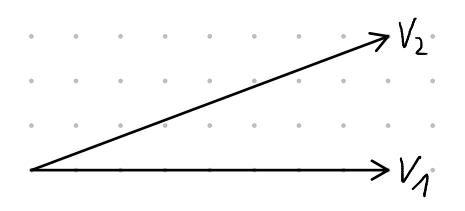
\includegraphics[width=0.25\textwidth]{Bild004}
            \caption{Problemstellung}
        \end{figure}

        $w_2=v_2-\frac{\langle v_2,v_1 \rangle_2}{\langle v_1,v_1 \rangle_2}v_1$ ist problematisch, falls $v_1\approx v_2$ (Auslöschung).
        Beim Gram-Schmidt-Verfahren können Rundungsfehler auftreten. Es ist instabil.

        \underline{\textbf{Ziel:}} Stabiler Algorithmus um $QR$-Zerlegungen zu berechnen.

    \section{Grundüberlegungen zu Orthogonalisierungsverfahren}

        \underline{\textbf{Problemstellung:}} Gegeben $v_1=\alpha e_1\in\R^2,v_2\in\R^2$ transformiere $v_2$ auf $\tilde{w_2}=\beta e_2$, gebe $\beta$ an.

        \underline{\textbf{Gram-Schmidt:}} $\beta=\left\Vert w \right\Vert_2$

        \begin{figure}[H]
            \centering
            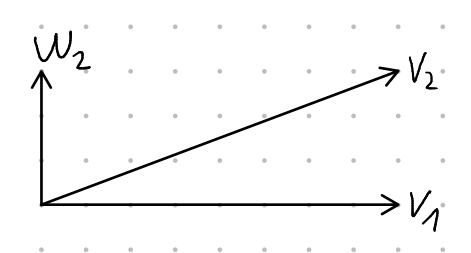
\includegraphics[width=0.25\textwidth]{Bild005}
            \caption{Gram-Schmidt}
        \end{figure}


        \underline{\textbf{Drehungen:}} $\tilde{w}_2= Qv_2$
        \[Q=\begin{bmatrix}
            \cos(-\theta) & \sin(-\theta) \\
            -\sin(-\theta) & \cos(-\theta)
        \end{bmatrix}\]
        \[\beta = \left\Vert v_2 \right\Vert_2\]

        \begin{figure}[H]
            \centering
            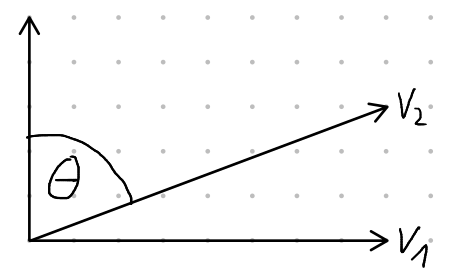
\includegraphics[width=0.25\textwidth]{Bild006}
            \caption{Drehungsansatz}
        \end{figure}


        \underline{\textbf{Spiegelungen:}} $\tilde{w}_2=Qv_2$, $Q=I-2\frac{vv^t}{v^tv}$ und $\beta=\left\Vert v_2 \right\Vert_2$

        \begin{figure}[H]
            \centering
            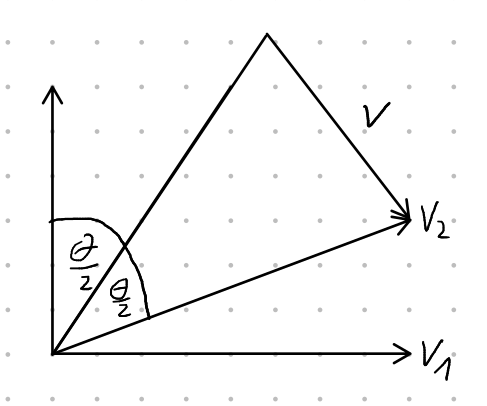
\includegraphics[width=0.25\textwidth]{Bild007}
            \caption{Spiegelungsansatz}
        \end{figure}


        \underline{\textbf{Idee:}} Benutze orthogonale Transformationen $Q_1,\dots,Q_n$ um $A\in\R^{m\times n}$ 
        ,$\rang(A)=n$, sukzessive zu reduzieren.
        \[A\rightsquigarrow Q_1A\rightsquigarrow Q_2Q_1 A\rightsquigarrow\dots\rightsquigarrow \begin{bmatrix}
            &R_1\\
            0 &\\
            \\
            & 0 &
        \end{bmatrix}\]

        Weil $\cond_2(Q)=1$ ist die Vorgehensweise stabil, bzw. gut konditioniert.

        \underline{\textbf{Aber:}} Wie wählen wir $Q_1,\dots,Q_n$?

    \section{$QR$-Zerlegung mittels Givens-Rotationen}

        \begin{definition}\label{d2.12}
            Eine Matrix der Form
            
            \[
                \delta_{k,l}=\begin{bmatrix}
                    1 & & & & & & & & \\
                    & \ddots & & & & & & & \\
                    & & c & &  & s & & & \\
                    & & & 1 &  & & & & \\
                    & & & &  \ddots  & & & & \\
                    & & -s & & & c & & & \\
                    & &  & & & & 1 & & \\
                    & &  & & & & & \ddots & \\
                    & &  & & & & &  & 1\\
                \end{bmatrix}
            \]
            , wobei die $s,c$ Einträge in der $k,l$ten Zeile / Spalte sind, heißen Givens-Rotationen.
        \end{definition}

        \underline{\textbf{Bemerke:}} Für $c=\cos(\theta),s=\sin(\theta)$ ist $\delta_{k,l}$ eine Drehung um $\theta$ in 
        in der Koordinaten $(k,l)$. $\delta_{k,l}$ ist Orthogonal.

        \underline{\textbf{Frage:}} Wie wählen wir $c,s$? 
        
        Gegeben $x\in\R^n$, elemeniere $l$te Koordinate zu $0$.

        \[\begin{bmatrix}
            c & s\\ -s & c
        \end{bmatrix}=\begin{bmatrix}
            x_k\\ x_l
        \end{bmatrix}=\begin{bmatrix}
            r\\0
        \end{bmatrix}\]

        \begin{figure}[H]
            \centering
            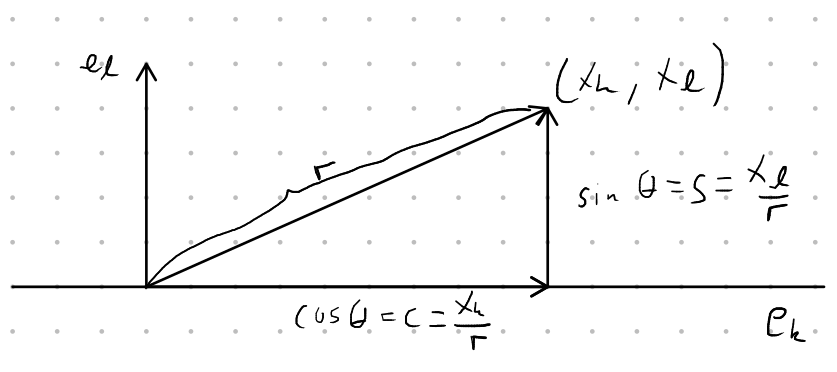
\includegraphics[width=0.25\textwidth]{Bild008}
            \caption{Trigonometriesetting}
        \end{figure}

        \begin{equation*}
            r^2=x_k^2+x_l^2
            \implies \pm \sqrt{x_k^2+x_l^2}
        \end{equation*}

        \underline{\textbf{Aber:}} Diese Berechnungsweise ist nicht unbedingt stabil ($x_k\gg x_l$)

        Stabile Variante:


        \begin{equation}\label{e2.3}
            \begin{array}{c}
                \text{Falls }\left\vert x_l \right\vert>\left\vert x_k \right\vert\implies \tau =\frac{x_k}{x_l},s=\frac{1}{\sqrt{1+\tau^2}},c=s\tau\\
                \text{Sonst: }\tau=\frac{x_l}{x_k},c=\frac{1}{\sqrt{1+\tau^2}},s=c\tau
            \end{array}
        \end{equation}
       

        Beispielprozess:

        \[
        \begin{bmatrix}
            * & * & * \\
            * & * & * \\
            \color{red}* & * & * \\
            \color{red}* & * & * \\
        \end{bmatrix}
        \rightsquigarrow
        \begin{bmatrix}
            * & * & * \\
            \color{red}* & * & * \\
            \color{red}* & * & * \\
            0 & * & * \\
        \end{bmatrix}
        \rightsquigarrow
        \begin{bmatrix}
            \color{red}* & * & * \\
            \color{red}* & * & * \\
            0 & * & * \\
            0 & * & * \\
        \end{bmatrix}
        \rightsquigarrow
        \begin{bmatrix}
            * & * & * \\
            0 & * & * \\
            0 & 0 & * \\
            0 & 0 & 0 \\
        \end{bmatrix}
        \]

        \begin{algorithm}[H]\label{a2.13}
            \caption{}
            \textbf{Input:} $A\in\R^{m\times n},m\geq n$\\
            \textbf{Output:} $R$ von der $QR$-Zerlegung ($A$ wird zerstört ``in place'')
            \begin{algorithmic}
            \For{$j=1,\dots, n$}
                \For{$i=m,m-1,\dots, j+1$}
                    \State Berechne $c,s$ wie in (\ref{e2.3})
                    \State $A[i-1:i,j:n]=\begin{bmatrix}
                        c & s \\
                        -s & c 
                    \end{bmatrix}^t A[i-1:i,j:n]$
                \EndFor
            \EndFor
            \end{algorithmic}
        \end{algorithm}

        \underline{\textbf{$m\approx n$:}}
    
        $c,s$: In jedem Eintrag einmal Wurzeln ziehen: $\implies \frac{n^2}{2}$ Quadratwurzeln und $\frac{4n^3}{3}$ Multiplikationen

        \underline{\textbf{$m\gg n$:}} $m\cdot n$ Quadratwurzeln und $2m\cdot n^2$ Multiplikationen

        \begin{remark}\label{r2.14}
            Der Algorithmus \ref{a2.13} berechnet nur $R$ von der $QR$-Zerlegung. Zur Berechnung von $Q$ müssten 
            zusätliche Operationen investiert werden um die Givens-Rotation auf $I$ anzuwenden.

            Für das lineare Ausgleichsproblem benötigen wir $Q^tb$, weshalb wir den Algorithmus auf $\left[\begin{array}{c|c}
                A & b
            \end{array}\right]$ anwenden können (da $R=Q^t A$).
        \end{remark}

        \begin{remark}\label{b2.15}
            Für $m=n$ ist die $QR$-Zerlegung eine (teure) ALternative zur $LR$-Zerlegung.
        \end{remark}

    \section{$QR$-Zerlegung mittels Householder-Transformationen}

        \begin{definition}\label{d2.16}
            Für $v\in\R^n,v\neq 0$, heißt \[Q=I-2\frac{\overbrace{vv^t}^{\in\R^{n\times n}}}{\underbrace{v^tv}_{\in\R}}\]
            Householder-Transformation / Reflexion / Spiegelung.
        \end{definition}

        \begin{tcolorbox}[enhanced,breakable,
            title=Wichtig!]
            Nicht $vv^t$ berechnen, das ist sehr uneffizient!
        \end{tcolorbox}

        Für $a,v\in\R^n,v\neq 0$ ist $Qa=\left(I-2\frac{vv^t}{v^tv}\right)a =a-2\frac{\langle v,a \rangle_2}{\langle v,v \rangle_2}v$

        \begin{figure}[H]
            \centering
            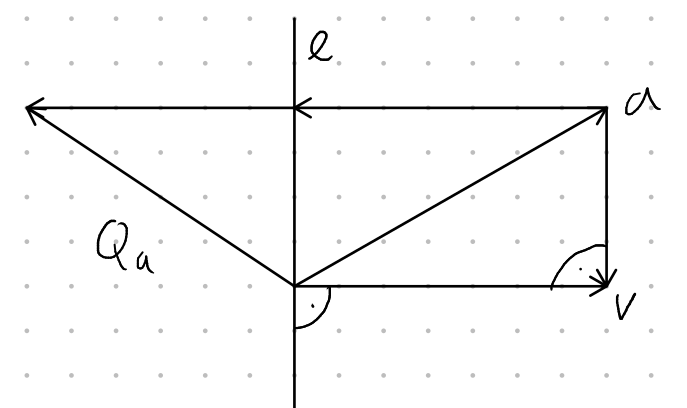
\includegraphics[width=0.25\textwidth]{Bild009}
            \caption{Householder-Transformationssetting}
        \end{figure}

        $Qa$ ist $a$ an $l$ gespiegelt.

        \begin{lemma}\label{l2.17}
            Für eine Householder-Transformation $Q\in\R^{n\times n}$ gilt:
            \begin{enumerate}
                \item $Q$ ist symmetrisch
                \item $Q$ ist orthogonal
                \item $Q$ ist involutionisch (eine Involution), d.h. $Q^2=I$
            \end{enumerate}
        \end{lemma}
        \begin{proof} % TODO
            Nachrechnen.
        \end{proof}

        \underline{\textbf{Frage:}} Gegeben $a\in\R^n$, wie müssen wir $v$ wählen, so dass $Qa=\alpha e_1$ für $\alpha\in\R$?

        % TODO? Kommentar Skalarprodukt etc. schnell auf PCs

        \underline{\textbf{Beobachte:}}

        \begin{enumerate}
            \item $\left\vert \alpha \right\vert=\left\Vert \alpha e_1 \right\Vert_2 = \left\Vert Qa \right\Vert_2 = \left\Vert a \right\Vert_2$
            \item $a\underbrace{-2\frac{\langle v,a, \rangle}{\langle v,v \rangle}}_{\in\R}v=Qa$
        
            $\implies v\in\text{span}(\alpha e_1-a) \implies \alpha =\pm\left\Vert a \right\Vert_2$ % ??

            Vermeide Auslöschung $\implies \alpha=-\text{sign}(a_1)\cdot\left\Vert a \right\Vert_2$
        \end{enumerate}

        \underline{\textbf{Effiziente Berechnung:}} Beobachte:
        \begin{align*}
            \left\Vert v \right\Vert_2^2 = \langle v,v \rangle_2 &= \langle  a-\alpha e_1, a-\alpha e_1  \rangle_2&\\
            &=\left\Vert a \right\Vert_2^2-2\alpha a_1 +\alpha^2&\\
            &=-2\alpha(a_1-\alpha)&\\
            \implies Qa &= a-2\frac{\langle v,a \rangle_2}{\left\Vert v \right\Vert_2^2}=a+\frac{\langle v,a \rangle_2}{\alpha(a_1-\alpha)}v&
        \end{align*}

        \noindent
        \xrfill[0.7ex]{1pt}Ende von Vorlesung 03 am 18.10.2022\xrfill[0.7ex]{1pt}
        
        \begin{lemma}\label{l2.18}
            Sie $\alpha\in\R^n,a\neq 0,a\notin\text{span}\{e_1\}$. 
            Sei \begin{equation}\label{g2.4}
                v=a-\alpha e_1,\alpha =-\text{sign}(a_1)\cdot \left\Vert a \right\Vert_2
            \end{equation} % oder alpha e_1-a
            Dann ist
            \begin{equation}\label{g2.5}
                \left(I-2\frac{vv^t}{v^tv}\right)a=a+\frac{v^ta}{\alpha(a_1-\alpha)}v=\alpha e_1.
            \end{equation}
        \end{lemma}

        \begin{proof}
            Siehe oben.
        \end{proof}

        \begin{algorithm}[H]\label{a2.19}
            \caption{}
            \textbf{Input:} $A\in\R^{m\times n},m\geq n$ ``Mehr Zeilen als Spalten''\\
            \textbf{Output:} $A\in\R^{m\times n}$, obere rechte Dreiecksmatrix $R$, Rest Householder-Transformationen
            \begin{algorithmic}
            \For{$j=1,\dots, n$} \Comment Iterieren über die Spalten
                \State Berechne $v,\alpha$ wie in (\ref{g2.4}) ,mit $a=A[j:m,j]\in\R^{m-j+1}$
                \State $v=\frac{1}{v_1}v$ \Comment Erster Eintrag wird nicht gespeichert, daher normalisieren wir
                \State Berechne $A[j:m,j:n]=\left(I-\frac{vv^t}{v^tv}\right)A[j:m,j:n]$ wie in (\ref{g2.5})
                \If{$j<m$}
                    \State A[j+1:m,j]=v[2:m-j+1]\Comment Index startet von 1 
                \EndIf
            \EndFor
            \end{algorithmic}
        \end{algorithm}

        \begin{remark}\label{b2.20}
            Die Skalierung $v=\frac{1}{v_1}v$ stellt sicher, dass die der erste Eintrag von $v$ nicht gespeichert werden muss.
        \end{remark}

        \underline{\textbf{Aufwand:}} $m\sim n \rightsquigarrow \frac{2}{3}n^3$ Multiplikationen

        $m\gg n \rightsquigarrow 2n^2m$ Multiplikationen

        Schneller als Givensrotationen, stabiler als Normalengleichungen

    \section{Pseudoinverse}

        \underline{\textbf{Ausgangspunkt:}} Wir wollen ein stabiles numerisches Verfahren, dass 
        \[
            Ax=b,A\in\R^{m\times n},m\geq n,\rang(A)=n,b\in\R^n    
        \]
        ``lösen'' kann, d.h. es gilt 
        \[
            \left\Vert Ax-b \right\Vert_2=\min_{y\in\R^n}\left\Vert Ay-b \right\Vert_2    
        \]

        Mathematisch können wir die Abbildung $b\mapsto x$, wegen der Normalengleichung (\ref{g2.2}), schreiben als 
        \[
            x=\underbrace{(A^tA)^{-1}A^t}_{\coloneqq A^\dagger}b=A^\dagger b    
        \]
        $A^\dagger\in\R^{n\times m}$. Wegen $A^\dagger A=I$ heißt $A^\dagger$ auch \textbf{Pseudoinverse}.

        \underline{\textbf{Frage:}} Können wir den Begriff der Inversen noch weiter verallgemeinern? Auf beliebige Matrizen?

        Satz \ref{s1.9}: $A\in\R^{m\times n}, U=\text{Bild}(A)$

        \begin{align*}
            &\implies \left\Vert Ax-b \right\Vert_2=\min_{y\in\R^n} \left\Vert Ay-b \right\Vert_2 \stackrel{\text{Satz \ref{s1.9}}}{\iff} Ax-b\in\text{Bild}(A)^\perp\\
            &\iff Ax- Pb -\underbrace{(b-Pb)}_{\in U^\perp:\text{ Satz \ref{s1.9}}}\in\text{Bild}(A)^\perp, Pb \text{ ist die orthogonale Projektion von } b \text{ auf } U\\
            &\iff \underbrace{\underbrace{Ax}_{\in U}-\underbrace{Pb}_{\in U}}_{\in U}\in\text{ Bild}(A)^\perp\\
            & \iff Ax=Pb
        \end{align*}

        Falls $\rang(A)<n$ (z.B., falls $m<n$) ist $Ax=Pb$ nicht eindeutig lösbar (aber es existiert immer eine Lösung).

        Für $\tilde{x}\in\R^n$ mit $A\tilde{x}=Pb,x'\in\text{ker}(A)$ ist $A(\tilde{x}+x')=Pb$.

        \begin{align*}
            L(b)&=\left\{x\in\R^n:\left\Vert Ax-b \right\Vert_2 = \min_{y\in\R^n} \left\Vert Ay-b \right\Vert_2\right\}\\
            &=\{x\in\R^n:Ax=Pb\}\\
            &=\tilde{x}+\ker(A)
        \end{align*}

        Sind gewisse Lösungen sinnvoller als andere?

        Wähle: $x\in\tilde{x}+\ker(A)$ mit minimaler Norm als ``eindeutige'' Lösung von $Ax=b$.

        \begin{align*}
            \stackrel{\text{Bem. \ref{b1.13}}}{\implies} \left\Vert x-0 \right\Vert_2 = \min_{y\in \tilde{x}+ \ker(A)} \left\Vert y-0 \right\Vert_2 &\iff x\in (\tilde{x}+\ker(A))^\perp \\
            &\iff x\in \ker(A)^\perp % TODO: Überprüfen    
        \end{align*}
        
        \begin{figure}[H]
            \centering
            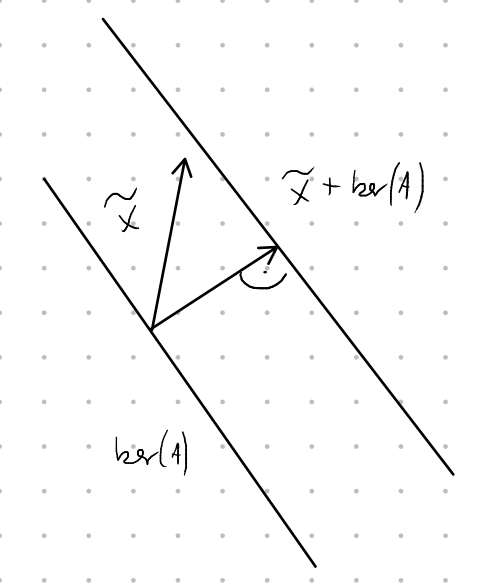
\includegraphics[width=0.25\textwidth]{Bild010}
            \caption{Setting}
        \end{figure}

        \begin{remark}\label{b2.21}
            Diese Wahl von $x$ für $b\mapsto x$ ist linear: Für $b_1,b_2\in\R^m$ ist:
            \[
            \begin{rcases*}
            Ax_1 = b_1 & $x_1 \in\text{ker}(A)^\perp$ \\
            Ax_2 = b_2 & $x_2 \in\text{ker}(A)^\perp$
            \end{rcases*} \implies P(x_1+x_2)=P(x_1)+P(x_2)=Ax_1+Ax_2=A(x_1+x_2),x_1+x_2\in \ker(A)^\perp
            \]
        \end{remark}

        \begin{definition}\label{d2.22}
            Sei $A\in\R^{m\times n}$. Die Abbildungsmatrix $A^\dagger\in\R^{n\times m}$ von $b\mapsto x$ heißt 
            \textbf{Pseudoinverse} oder \textbf{Moore-Pensore-Inverse} von $A$. D.h. gegeben $b\in\R^n$, dann ist $x=A^\dagger b$ die eindeutige Lösung von 
            \[
                \min_{y\in\ker(A)^\perp} \left\Vert Ay-b \right\Vert_2 = \left\Vert Ax-b \right\Vert_2.    
            \]
        \end{definition}
        
        \begin{theorem}\label{s2.23}
            $A\in\R^{m\times n}$. Dann ist $A^\dagger\in\R^{m\times n}$ eindeutig über die Moore-Penrose-Axiome definiert:
            \begin{enumerate}
                \item $(A^\dagger A)^t=AA^\dagger$
                \item $(AA^\dagger )^t=A^\dagger A$
                \item $A^\dagger AA^\dagger = A^\dagger$
                \item $AA^\dagger A=A$
            \end{enumerate}
        \end{theorem}

        \begin{proof}
            Siehe Literatur oder später
        \end{proof}

        \underline{\textbf{Frage:}} Wie berechnen wir $x=A^\dagger b$?

        Sei $A\in\R^{m\times n},\rang(A)=p\leq \min(m,n)$. Bringe $A$ mittels orthogonaler Transformationen (z.B. Householder) auf 
        obere Dreiecksgestalt, d.h.:

        \begin{equation}\label{g2.6}
            Q^tA=\begin{bmatrix}
                &  &  & & & \\
                & R & & S & & \\
                * & & & & &\\
                & 0 & &  0 & & \\ 
            \end{bmatrix}
        \end{equation}
        wobei  $S\in \R^{p\times (n-p)}$.
        Setze Analog $x=\begin{bmatrix}
            x_1\in\R^p\\
            x_2\in R^{n-p}
        \end{bmatrix},Q^t b=\begin{bmatrix}
            b_1\in\R^p\\
            b_2\in \R^{m-p}
        \end{bmatrix}$

        \begin{lemma}\label{l2.24}
            Mit obigen Bezeichungen ist $x=A^\dagger b$ genau dann, wenn \[x_1=R^{-1}b_1-R^{-1}Sx_2.\]
        \end{lemma}
        \begin{proof}
            \begin{align*}
                \left\Vert Ax-b \right\Vert_2^2&=\left\Vert Q^t(Ax-b) \right\Vert_2^2\\
                &=\left\Vert \begin{pmatrix}
                    Rx_1+Sx_2-b\\
                    -b_2
                \end{pmatrix} \right\Vert_2^2\\
                &= \left\Vert Rx_1+Sx_2 -b_1\right\Vert_2^2+\left\Vert b_2 \right\Vert_2^2
            \end{align*}
            ist minimal, falls $Rx_1=b_1-Sx_2$.
        \end{proof}

        Wir sehen $p=\rang(A)=n\implies$ wie vorher, lineares Ausgleichsproblem!

        Sonst: $x_2=$?

        \begin{lemma}\label{l2.25}
            Sei $p<n,V=R^-1S\in\R^{n\times (n-p)}$ und $u=R^{-1}b_1\in\R^p$. Dann ist
            \begin{align*}
                x&=A^\dagger b\\
                \iff &(I+V^tV)x_2=V^tu\\
                &x_1=u-Vx_2
            \end{align*}
        \end{lemma}

        \begin{proof}
            \begin{align*}
                \left\Vert x \right\Vert_2^2 &= \left\Vert x_1 \right\Vert_2^2 + \left\Vert x_2 \right\Vert_2^2\\
                &\stackrel{\text{Lemma \ref{l2.24}}}{=}\left\Vert u-Vx_2 \right\Vert_2^2+ \left\Vert x_2 \right\Vert_2^2\\
                &=\left\Vert u \right\Vert_2^2-2 \langle u,Vx_2 \rangle_2+\langle Vx_2,Vx_2 \rangle_2+\langle x_2,x_2 \rangle_2\\
                &=\left\Vert u \right\Vert_2^2+\langle x_2,(I+V^tV)x_2-2V^tu \rangle_2 = \varphi(x_2)
            \end{align*}
            Minimiere $\varphi(x_2)$:
            \begin{align*}
                \varphi'(x_2)=-2V^tu+2(I+V^tV)x_2\\
                \varphi'(x_2)=2(I+V^tV) \implies \text{spd}
            \end{align*}
            $\varphi$ minimal $\iff \varphi'(x_2)=0\implies $ Behauptung.
        \end{proof}

        \begin{algorithm}[H]\label{a2.26}
            \caption{}
            \textbf{Input:} $A\in\R^{m\times n},b\in\R^m$\\
            \textbf{Output:} $x=A^\dagger b$
            \begin{algorithmic}
            \State Berechne $QR$-Zerlegung (\ref{g2.6}) von $A$
            \State $\begin{bmatrix}b_1\\b_2\end{bmatrix}=Q^t b$
            \State $V=R^{-1}S$ mittels Rückwertssubstitution 
            \State $u=R^{-1}b_1$ mittels Rückwertssubstitution
            \State Löse $(I+V^tV)x_2=V^tu$ mittels Cholesky-Zerlegung 
            \State $x_1=u-Vx_2$
            \State $x=\begin{bmatrix}x_1\\x_2\end{bmatrix}$
            \end{algorithmic}
        \end{algorithm}

        \noindent
        \xrfill[0.7ex]{1pt}Ende von Vorlesung 04 am 20.10.2022\xrfill[0.7ex]{1pt}
        

\end{document}